%%%%%%%%%%%%%%%%%%%%%%%%%%%%%%%%%%%%%%%%%%%%%%%%%%%%
%%%% En-tête leçon
\begin{headerBlock}
  \chapter{Phénomènes interfaciaux impliquant des fluides}
    \label{LP_PhenomenesInterfaciaux}
\end{headerBlock}




%%%%%%%%%%%%%%%%%%%%%%%%%%%%%%%%%%%%%%%%%%%%%%%%%%%%
%%%% Références
\begin{center}
\begin{tabularx}{\textwidth}{| X | X | c | c |}
  \hline
  \rowcolor{gray!20}\multicolumn{4}{c}{Bibliographie de la leçon : } \\
  \hline 
  Titre & Auteurs & Editeur (année) & ISBN \\
  \hline
 Gouttes, bulles, perles et ondes & David Quéré, Françoise Brochard-Wyart et Pierre-Gilles de Gennes & \'Editions Belin (2002) &    \\
  \hline 
 Hydrodynamique physique & \'Etienne Guyon, Jean-Pierre Hulin et Luc Petit  &  CNRS ÉDITIONS (3ème édition) &    \\
  \hline 
  Capillarité (cours) & P. Lidon  & \url{https://cel.hal.science/cel-01332274} &  \\
  \hline
Notes de cours sur les fluides (2019-2020) & Marc Rabaud  &  Site agreg Montrouge  &    \\
  \hline 
 Why is surface tension a force parallel to the interface? & Marchand, A., Weijs, J. H., Snoeijer, J. H., \& Andreotti, B   & American Journal of Physics (2011)  &    \\
  \hline
\end{tabularx}
\end{center}

%%%%%%%%%%%%%%%%%%%%%%%%%%%%%%%%%%%%%%%%%%%%%%%%%%%%

%%%%%%%%%%%%%%%%%%%%%%%%%%%%%%%%%%%%%%%%%%%%%%%%%%%%
%%%% Plan
\begin{reportBlock}{Plan détaillé}

  \textbf{Niveau choisi pour la leçon :} License 3
  \newline
  \textbf{Prérequis} : \begin{itemize}
      \item Forces, travaux de force, énergie
      \item Principe de travaux virtuels
      \item Equation de l'hydrostatique
  \end{itemize}

  
  \textbf{Déroulé détaillé de la leçon: }   \newline
  
  \section*{Introduction (3min)}
L'étude des phénomènes interfaciaux permet de répondre à un certain nombre de questions comme : pourquoi est-ce que insectes marchent sur l'eau, pourquoi les gouttes et les bulles ont la formes qu'elles ont, ou encore pourquoi en TP de chimie, lorsqu'on met un liquide dans un tube, on voit la formation d'un ménisque ?
  \section{Tension de surface}
  \subsection{Définition}
  \textcolor{purple}{Expérience qualitative films de savon sur des surfaces (cubes) : il faut que le système minimise son énergie de surface.}\\
  Si on augmente la surface d'une interface \textit{dA}, le coût en énergie associé vaut : 
  \begin{equation}
      \delta W = \gamma dA
  \end{equation}
  avec $\gamma$ le coefficient de tension de surface (J.m$^{-2}$). C'est l'énergie qu'il faut fournir pour augmenter la surface d'une interface d'une unité. Ex : pour l'interface eau-air, $\gamma = 72.8$~mJ/m$^2$ à $20^{\circ}$C. 
  
  \subsection{Origine microscopique}
  Une molécule en volume subit des interactions de cohésion de la part de ses voisines qui la stabilisent. Une molécule à l'interface n'a plus de voisines au dessous, cette configuration augmente son énergie. Le fluide ajuste donc sa forme pour exposer le minimum de surface afin de minimiser son énergie.

  La forme minimale pour une goutte ou une bulle en l'absence d'interaction est une sphère (vidéo bulle d'eau dans l'espace : \url{https://www.youtube.com/watch?v=bKk_7NIKY3Y}). 
  
  \subsection{Force capillaire (7min)}
  Le coefficient de tension de surface peut également être vu comme une force par unité de longueur. \\
  Vidéo force capillaire \url{https://www.youtube.com/watch?v=g4c_tj1CccE}.
  Permet de répondre à pourquoi le gerris peut marcher sur l'eau: les pattes hydrophobes du gerris déforment la surface de l'eau qui va chercher à retrouver sa forme en appliquant une force capillaire sur les pattes. Comme l'insecte est suffisamment léger, la force arrive à compenser le poids. 
  
 \subsection{Pression et tension de surface}
 Question : La pression est-t-elle plus grande dans les petites bulles ou dans les grandes bulles ? \\
 \textcolor{purple}{Expérience avec générateur de bulles : la petite bulle est "mangée" par la grosse.}
 \begin{center}
     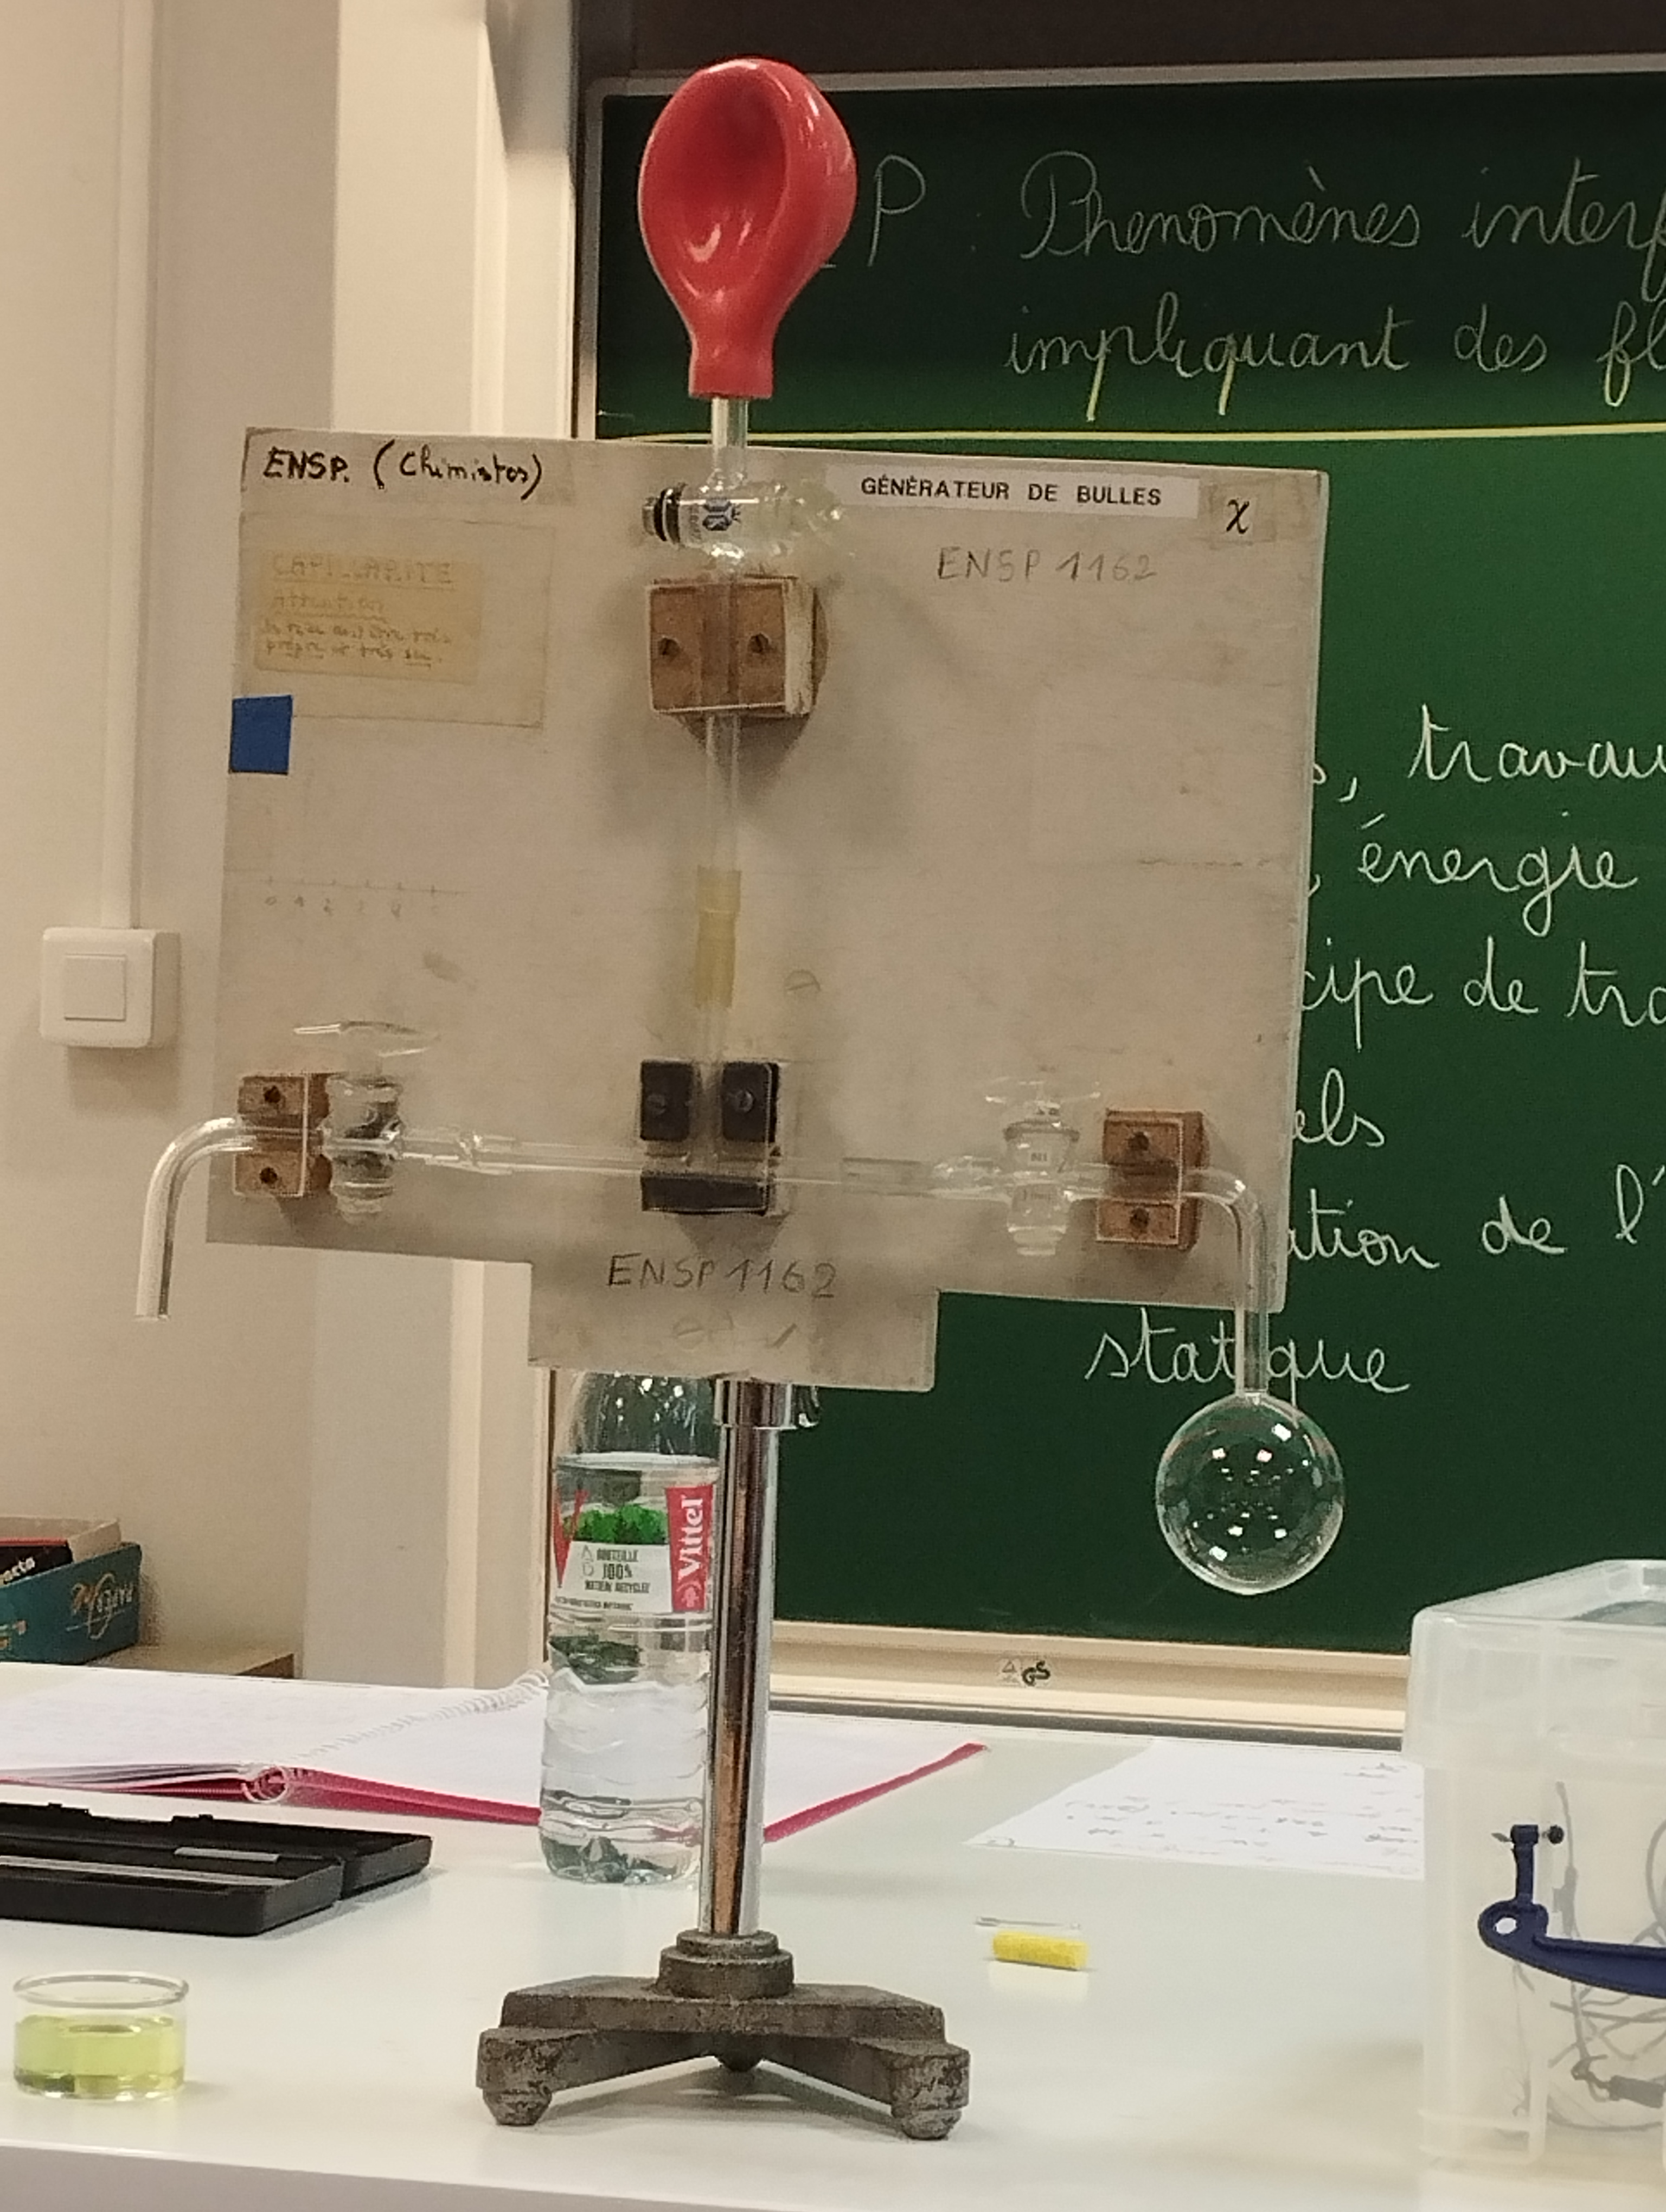
\includegraphics[scale=0.1]{LP_TensionSurface/Manip_Laplace.jpg}
     
 \end{center}
 CCL : la pression est donc plus grande dans les petites bulles : on peut le démontrer mathématiquement via la \textbf{Loi de Laplace.}
 Pour cela, on applique le principe des travaux virtuels. On imagine que l'on déforme une bulle de $dR$ : \\
 $\delta W = -P_1dV_1-P_2dV_2+\gamma dA =0$ à l'équilibre.\\
 $\ud V_1 = - \ud V_2 = 4 \pi R^2 \ud R$\\
 $dA = d(4\pi R^2) = 8\pi RdR$.\\
 Finalement : 
 \textcolor{red}{Loi de Laplace : }
 \begin{equation}
     (P_1-P_2)=\frac{2\gamma}{R}
 \end{equation}
 \begin{itemize}
     \item Plus $R$ est petit, plus la pression à l'intérieur est grande. 
     \item Lorsque $R \rightarrow \infty$ (surface plane), on a continuité de la pression.
     \item Cette loi nous permet de mesurer $\gamma$ expérimentalement.
 \end{itemize}
 \subsection{Mesure de $\gamma$ (17min)}
 \textcolor{purple}{Expérience :}  Pour une bulle de savon, deux interfaces donc $\Delta P =\frac{4\gamma}{R}$. On génère une bulle, on mesure son rayon et la pression à l'intérieur grâce à un manomètre différentiel de mesurer la différence de pression entre l'intérieur de la bulle et l'extérieur à travers une mesure de tension (piézo). J'ai pris plusieurs points en préparation, je vais en prendre un devant vous. Une regression linéaire $\delta P = \frac{A}{R}$ permet d'obtenir $\gamma$. \\
 \textbf{19min30}\\

La pente de $\Delta P = 4 \gamma\times 1/R$ donne $\gamma=28.8 \pm 2.2$~mN/m$^2$ qui est plus faible que celle de l'eau dû à la présence d'un tensioactif (savon = tensioactif). Par ailleurs, on retrouve le bon ordre de grandeur pour une eau savonneuse (internet donne $25$~mN/m$^2$). \\


  \section{Contact à 3 phases : mouillage (22min)}
  \textcolor{green}{Mouillage :} étude de l'étalement d'une liquide sur un substrat (solide ou liquide). Utile dans l'industrie (peinture, encre, traitement des pneus, crème, maquillage, etc.).\\
  $\theta =$ angle de contact, permet de savoir si un liquide mouille plus ou moins bien un substrat. Résulte d'une compétition entre les tensions de surface intervenant dans les trois interfaces (L/G, L/S, S/G). \\
  \textbf{26min}\\
  Le système est \{\textbf{dl}$\in$ ligne triple\}. 
  $\textbf{dF}=0$ à l'équilibre. La projection sur l'axe du solide donne la \textcolor{red}{Loi de Young-Dupré} :
  \begin{equation}
      \gamma_{LG}\cos(\theta) = \gamma_{SG}-\gamma_{SL}
  \end{equation}
  
  \section{Influence de la gravité}
  On voit que plus la taille de la goutte est importante, plus la goutte est applatie : il y a un effet de gravité qui n'est plus négligeable à partir d'une certaine taille : laquelle ?
  \subsection{Nombre de Bond (30min)}
  Compétition entre gravité et tension de surface : $B_0=\frac{\rho R^2g}{\gamma}$. La longueur capillaire $l_c$ est telle que: $B_0=\frac{\rho l_c^2g}{\gamma}=1$ (frontière entre les deux régime), soit $l_c = \sqrt{\frac{\gamma}{\rho g}}$.
  Pour l'eau, $l_c=3$mm.\\
  Deux régimes : 
  \begin{itemize}
      \item $R>>l_c$, la gravité domine : goutte plate.
      \item $R<<l_c$, la tension de surface domine, la bulle est sphérique.
  \end{itemize}
  Photo ménisque : résulte de cette compétition entre tension de surface responsable de sa formation et gravité qui s'y oppose. Menisque concave pour un fluide mouillant (ex: eau dans tube en verre) et convexe pour un fluide peu mouillant (ex: mercure dans tube en verre)
  \begin{center}
      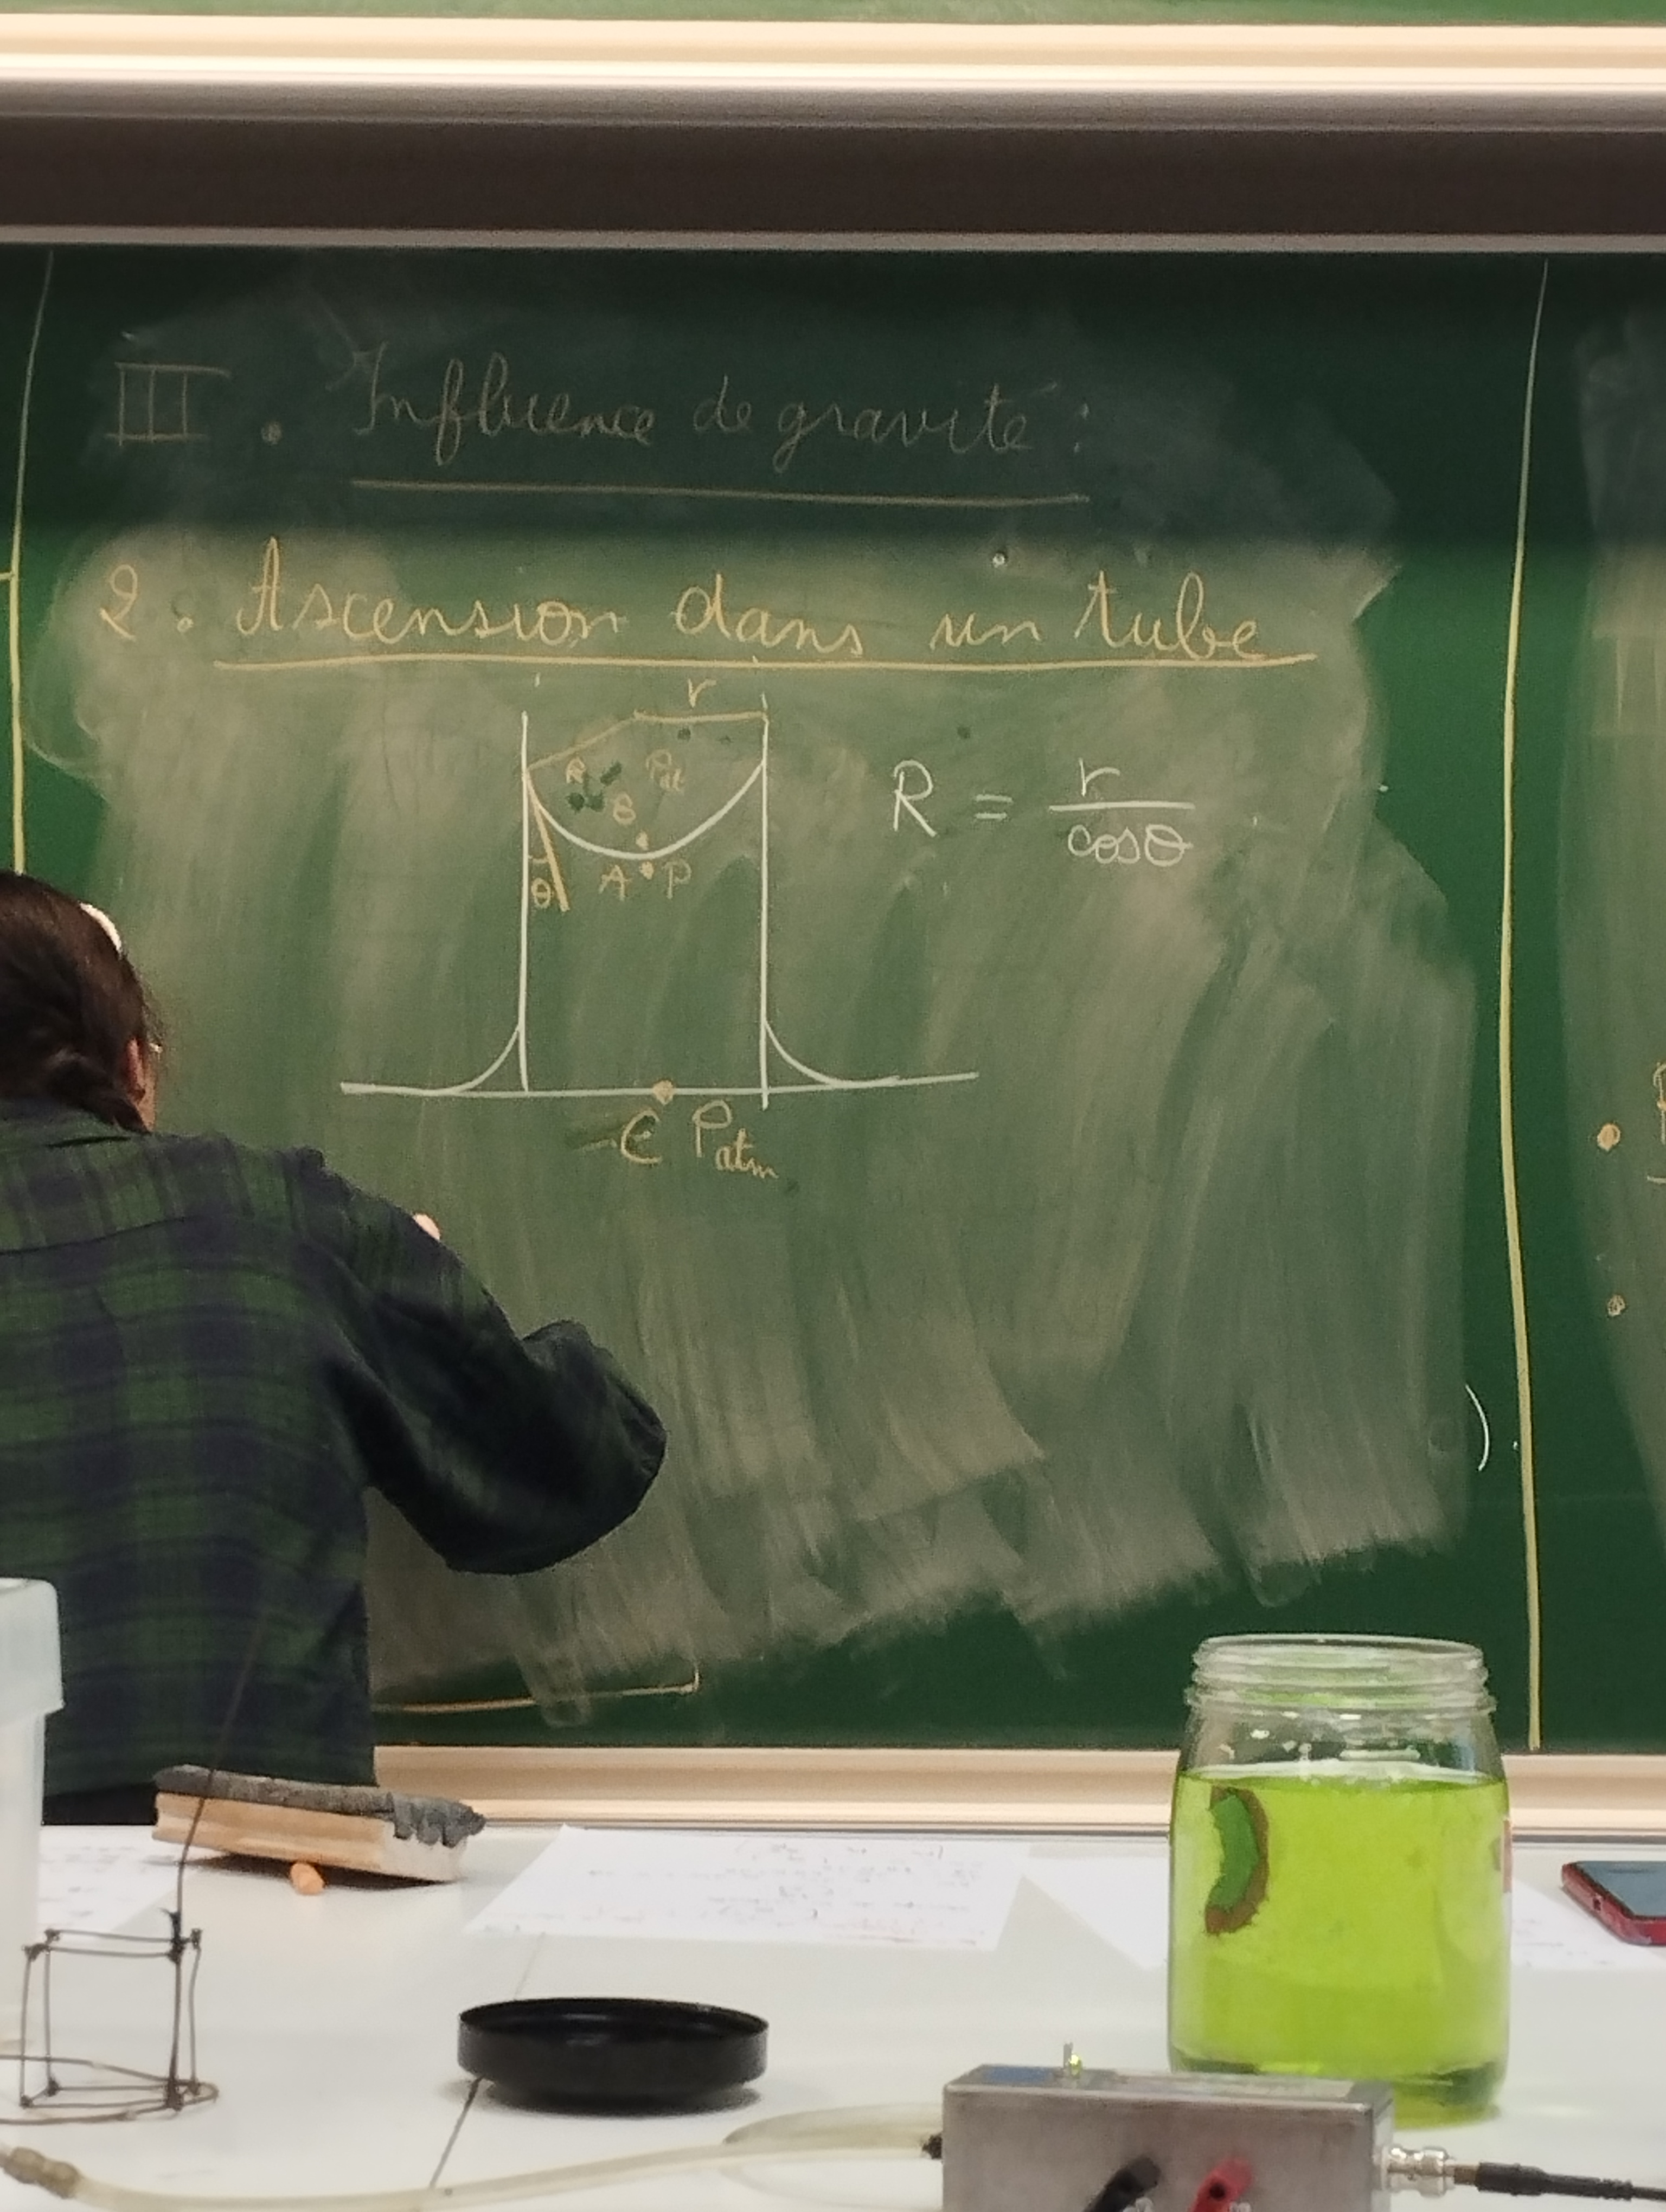
\includegraphics[scale=0.1]{LP_TensionSurface/Menisque.jpg}
  \end{center}

  \subsection{Ascension dans un tube (34min)}
  Vidéo de l'ascension d'un liquide dans différents tubes capillaires. Plus le tube est fin, plus le liquide monte haute.
  Schéma liquide dans un tube de rayon $r$, rayon de courbure du ménisque $R$, angle de contact $\theta$. On applique la loi de Laplace : $\Delta P = \frac{2\gamma}{R}=\frac{2\gamma\cos(\theta)}{r}$. En appliquant l'équation de l'hydrostatique, on obtient \textcolor{red}{la Loi de Jurin} :
  \begin{equation}
      h = \frac{2\gamma\cos(\theta)}{\rho g r}
  \end{equation}
  En effet, plus $r$ est petit, plus $h$ est grand. Cette loi permet de mesurer $\gamma$.
  
  \section*{Conclusion (40min)}
  Expérience de conclusion : Pince à nourrice dans eau flotte, puis coule avec tensio-actif (savon).



\end{reportBlock}


%%%%%%%%%%%%%%%%%%%%%%%%%%%%%%%%%%%%%%%%%%%%%%%%%%%%
%%%% Questions
\begin{reportBlock}{Questions posées par l’enseignant (avec réponses)}
  \textbf{C : C'est quoi un tensioactif ?} \textcolor{purple}{\'{E}lément qui diminue la tension de surface. Il est composé d'une tête hydrophile et d'une queue hydrophobe. La tête va se mettre à l'interface du côté de l'eau tandis que la queue sera du côté de l'air, faisant le lien entre l'eau et l'air. Cette configuration permet de diminuer l'énergie de l'interface, et donc diminue la tension de surface. } \newline

  \textbf{C : La dynamique de l'ascension dans la loi de Jurin semble diférrente en fonction du diamètre du tube ? Pouvez-vous discuter des éléments à prendre en compte pour essayer de comprendre pourquoi ça monte plus vite ou plus lentement ?} \textcolor{purple}{Plus le rayon est grand, plus la vitesse est grande. Peut se comprendre en ordre de grandeur via $\nabla P = \eta \Delta v$ soir $\frac{P}{h} \sim \eta \frac{v}{r^2}$}
  %En comparant à Poiseuille cylindrique, il y a une dépression à l'interface air/liquide qui fait augmenter brutalement la vitesse. Lorsque le liquide monte, le gradient de pression diminue ($\frac{\delta P}{\delta z}=\frac{2\gamma}{rh}$, r rayon du tube et h hauteur de l'ascension) et en prenant en compte la gravité et les forces de viscosité ($\frac{\delta^2v_r}{\delta z^2}$), ça va ralentir l'ascension.

  \textbf{C : Où placeriez-vous cette leçon dans le cours global de mécanique des fluides ?} \textcolor{purple}{Après l'équation de Navier-Stokes. C'est presque une domaine un peu à part.}

  \textbf{C : Peut-on imaginer qu'on n'ait pas de saut de pression à travers une surface courbe ?} \textcolor{purple}{En utilisant l'équation de Laplace pour une surface quelconque, $\Delta P =\gamma(1/R+1/R')$, R et R' sont les deux rayons de courbures de la surface en un point donné et sont algébriques (compté positivement si le centre de la coubure est à l'intérieur de la surface, négativement sinon. Par exemple, pour un point selle, on a $R' = -R$ impliquant une continuité de la pression.}

  \textbf{C : Dans l'équation de Young-Dupré, vous avez dessiné 3 forces mais il ne me semblait pas qu'on était en équilibre (au moins à la normale à la surface)} \textcolor{purple}{La force de réaction du support compense la composante normale de la force de tension de surface.}

  
  \textbf{C : D'autres façon pour déterminer $\gamma$ ?} \textcolor{purple}{Tensiomètre à plaque de Wilhelmy: on mesure la force exercée sur la plaque par le liquide grâce à une microbalance, et on peut en déduire $\gamma$.}

  
  \textbf{C : Dessin d'une goutte sur un plan incliné ? De quoi dépendrait l'angle d'inclinaison ?} \textcolor{purple}{Vitesse, viscosité, et coefficient de tension de surface.}

  
  \textbf{C : Pouvez-vous expliquer pourquoi on peut faire des chateaux de sables avec du sable mouillé ?} \textcolor{purple}{La présence d'eau va créer un pont capillaire entre deux grains qui va augmenter la force de cohésion entre les grains. Cette cohésion se fait sur une surface beaucoup plus grande pour le grain mouillée grâce au pont capillaire alors que pour un grain sec, cette cohésion se fait au niveau d'une rugosité (très petite surface) et donc insuffisance pour maintenir un château de sable.}



  \textbf{C : Pourquoi les serviettes sont rêches quand elle sèche ? Quel est le principe d"un adoucissant ?} \textcolor{purple}{Lorsqu'une serviette est mouillée, l'eau va chercher à minimiser son interface avec l'air en collant et écrasant les fibres de la serviette (c'est aussi pour ça que nos cheveux sont collés en sortant de la douche). En séchant, la serviette durcit, lui donnant une texture rêche. L'adoucissant agit chimiquement sur les fibres pour rendre le linge plus doux au toucher.}


  \textbf{C : $\gamma(T)$ ? Que se passe-t-il s'il y a des endroits du fluide qui sont plus chauds que d'autres ?} \textcolor{purple}{Création d'un gradient de tension de surface qui va causer un déplacement du liquide des zones de faibles $\gamma$ vers les zones de $\gamma$ élevée (cf. effet Marangoni).}

  
  \textbf{C : On parle parfois de liquide mouillant et de liquide non-mouillant. Valeurs de $\theta$ ?} \textcolor{purple}{Mouillage total : $\theta=0$, non-mouillage total : $\theta=\pi$.}

  
  \textbf{C : Commenter les incertitudes sur l'expérience ?} \textcolor{purple}{Incertitudes dominantes sur la mesure du rayon avec le pied à coulisse que j'ai pris de $0.5$mm, ce qui est une grande incertitude.}


  \textbf{C : Principe du manomètre ?} \textcolor{purple}{Un piézoélectrique subit une contrainte mécanique sous l'effet de la différence de pression, générant une tension que l'on mesure. Le constructeur nous donne la relation de conversion entre tension et pression.}

  \end{reportBlock}
  
%%%%%%%%%%%%%%%%%%%%%%%%%%%%%%%%%%%%%%%%%%%%%%%%%%%%
%%%% Commentaires
\begin{reportBlock}{Commentaires lors de la correction de la leçon}
Bonne leçon, beaucoup apprécié toutes les expériences montrées. Vous maîtrisez pas mal de choses. Attention à ce que le dispositif ne gène pas la vue sur le tableau.\\


\end{reportBlock}



%%%%%%%%%%%%%%%%%%%%%%%%%%%%%%%%%%%%%%%%%%%%%%%%%%%%
%%%% Correction
\begin{reportBlock}{Partie réservée au correcteur}
  \textbf{Avis général sur la leçon (plan, contenu, etc.) :}
  
  
  \textbf{Notions fondamentales à aborder, secondaires, délicates :}
  
  
  \textbf{Expériences possibles (en particulier pour l'agrégation docteur) :}
  
  
  \textbf{Bibliographie conseillée :}
\end{reportBlock}


\begin{reportBlock}{Partie réservée au correcteur}
  \textbf{Avis général sur la leçon (plan, contenu, etc.) :}
  
  
  \textbf{Notions fondamentales à aborder, secondaires, délicates :}
  
  
  \textbf{Expériences possibles (en particulier pour l'agrégation docteur) :}
  
  
  \textbf{Bibliographie conseillée :}
\end{reportBlock}